\documentclass[11pt]{report}
\usepackage{amsmath}
\usepackage{graphicx}

\title{Modeling and Simulation Hand In 3}
\author{Georgios Smyridis}

\begin{document}

\maketitle

\section*{Exercise 8)}

This exercise is concerned with a Monte Carlo simulation for a Lennard-Jones fluid in the NVT ensemble. The potential that is employed is the truncated and shifted Lennard-Jones potential between two particles $i$ and $j$ given by the relationship
\begin{align}
	u(r_{ij})=\left\{
	\begin{aligned}
		&4\epsilon \bigg[\bigg(\frac{\sigma}{r_{ij}}\bigg)^{12}-\bigg(\frac{\sigma}{r_{ij}}\bigg)^{6}\bigg] -e_{cut} \qquad r_{ij}\leq r_{cut} \\
		&0 \qquad\qquad\qquad\qquad\qquad\qquad\quad\quad r_{ij}\geq r_{cut}
	\end{aligned}
	\right.
\end{align}
where 
\begin{align}
	e_{cut} = 4\epsilon \bigg[\bigg(\frac{\sigma}{r_{cut}}\bigg)^{12}-\bigg(\frac{\sigma}{r_{cut}}\bigg)^{6}\bigg] 
\end{align}
and $r_{cut}$ is the cutoff radius. It is convenient to choose $\sigma$ as the unit of length, $\epsilon$ the unit of energy, and $m$ the unit of mass. For this exercise, we have to take a box with length of at least 2$r_{cut}$, which is fixed at $r_{cut}=2.5\sigma$. The reason is that we want to calculate the potential using the nearest image convention and this will be valid only if $r_{cut}$ is smaller than half the length of the box.

\subsection*{Question 1)}

We first calculate the average pressure using the virial equation for the pressure:
\begin{align}
	\left<P\right>=\rho k_BT+\frac1{3V}\left<\sum_{i<j}f(r_{ij})\cdot r_{ij}\right>
\end{align}
where the virial sum can be written in terms of the intermolecular force:
\begin{align}
	f(r)&=-\nabla u(r)=-\sum_{i=1}^3\frac{\partial u(r)}{\partial x_i}\hat x_i=-\sum_{i=1}^3\frac{\partial r}{\partial x_i}\frac{\partial u(r)}{\partial r}\hat x_i=-\frac{\partial u(r)}{\partial r}\hat r
\end{align}
Then, it is easy to carry the differentiation to come up with
\begin{align}
	f(r)\cdot r=24\epsilon\bigg[2\bigg(\frac{\sigma}{r}\bigg)^{12}-\bigg(\frac{\sigma}{r}\bigg)^6\bigg]
\end{align}
or, with our units
\begin{align}
	f(r)\cdot r = 24\bigg(2r^{-12}-r^{-6}\bigg)
\end{align}
Therefore, we can write a class measure() which contains a method that measures the quantity
\begin{align}
	\frac{\rho}{\beta}+\frac{8}{V}\sum_{i<j}\bigg(2 r^{-12}-r^{-6}\bigg)
\end{align}
and then, during our Monte Carlo simulation, calculate the averages.


\subsection*{Question 2)}

Now, I calculate the excess chemical potential using the Widom test particle method. This requires us to add a new particles in the system at a random place, calculate the change in the energy, that is, its energy contribution to the system's energy $\Delta U^+$. Then, we exponentiate this quantity with the corresponding Boltzman weight to calculate the excess chemical potential. To make the measurements statistically significant, we repeat the test NTEST times and average. That is,
\begin{align}
	\mu_{ex}=-k_BT\ln\bigg(\sum_{i=1}^{NTEST}\frac{\exp[-\beta\Delta U_i^+]}{NTEST}\bigg)
\end{align}
Instead of a dat file, I saved my results into a csv file, which is easier to work with.


\subsection*{Question 3)}

The Widom test along with the virial expression cannot be used to measure the average pressure of a system. The reason is that the interaction potential between two hard spheres is infinite if their distance is smaller than the diameter of the spheres, and zero otherwise. This means that inserting a sphere into the system can happen only if there are no overlaps and then, the potential of the system remains zero. Without calculating an difference in energy, we cannot use the Widom test.


\subsection*{Question 4)}

The plot of the system's pressure as a function of the density is in Figure 1.

\begin{figure}[ht!]
\begin{center}
	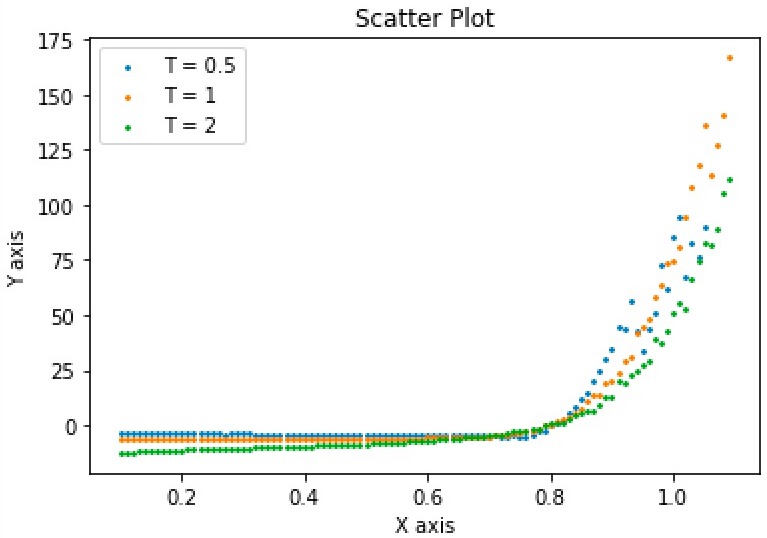
\includegraphics[scale = 0.4]{P.jpeg}
	\caption{Pressure -- Density}
\end{center}	
\end{figure}



\subsection*{Question 5)}

The ideal gas law is most accurate when the gas particles are at low densities or high temperatures. When a gas is at low density, the particles are far apart and their interactions become weaker. This means that the gas behaves more like an ideal gas, which is a theoretical gas that has no interparticle interactions. Similarly, at high temperatures, the kinetic energy of the gas particles increases and the thermal fluctuations become greater than the interparticle interactions. This makes the gas behave more like an ideal gas, where the particles move independently of one another. 

\subsection*{Question 6)}

The plot of the chemical potential $\mu$ as a function of density is in Figure 2.

\begin{figure}[ht!]
	\begin{center}
		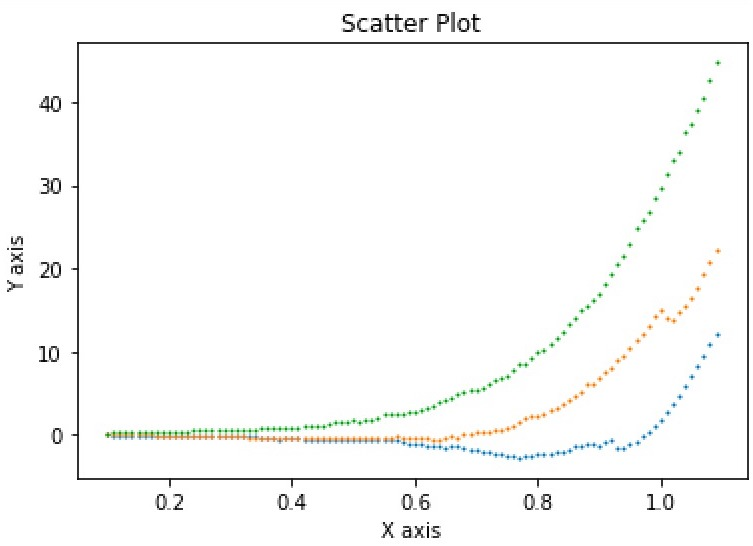
\includegraphics[scale = 0.4]{Mu.jpeg}
		\caption{Chemical Potential -- Density}
	\end{center}
\end{figure}

\end{document}
